\documentclass[12pt]{article}
\usepackage{geometry}
\usepackage{amsmath}
\usepackage{amsthm}
\usepackage{amssymb}
\usepackage{mathrsfs}
\usepackage{parskip}
\usepackage{enumerate}
\usepackage{stmaryrd}
\usepackage{listings}
\usepackage{fullpage}
\usepackage[x11names, rgb]{xcolor}
\usepackage[utf8]{inputenc}
\usepackage{tikz}
\usetikzlibrary{snakes,arrows,shapes}

\begin{document}

\title{CS 360 Notes}
\author{Matthew Visser}
\date{Nov  1, 2011}
\maketitle

Acceptance by final state:
\begin{equation}
	L(P) = \{w|(q_0,w,Z_0)\vdash_p^* (p,\varepsilon,\alpha) \text{ for some } p
	\in F, \alpha \in \Gamma^* \}
	\label{acceptFinal}
\end{equation}
Accept by empty stack:
\begin{equation}
	L(P) = \{w|(q_0,w,Z_0)\vdash_p^* (p,\varepsilon,\varepsilon) \text{ for any} p
	\in Q\}
	\label{acceptEmpty}
\end{equation}

\textbf{Theorem}: Suppose that $P_F$ is a PDA that accepts by final state. Then
there exists a PDA, $P_N$ that accepts the language $L(P_F)$ by empty stack.

\begin{proof}
	We can construct a PDA with a new start state and end state. For every end
	state in $P_F$, have a transition to the new final state.  The final state
	loops, popping elements off the stack until it's empty. We can prove by
	induction that this is correct.
\end{proof}

We also have a theorem for the other direction.

\textbf{Theorem}: Suppose that $P_N$ is a PDA that occepts by empty stack. There
exists a PDA $P_F$ that accepts $N(P_N)$ by final state.

\begin{proof}
	Change the stack at the start to $Z_0X_0$ with a new start state and a
	transition to the old start state.  For every state, we have a transition
	where if $X_0$ is on the top of the stack, we go to a new end state.
\end{proof}

\textbf{Theorem}: PDAs that accept by empty stack accept all of, and only,
context free-languages.
\textbf{Corollary}: PDAs that accept by final state also accept context-free
languages.

\begin{proof}
	Given a CFG $G$ whose language is $L$, we can create a PDA $P$ such that
	$N(P) = 1$

	Consider $S \to aSa | bSb | b | \varepsilon | a$

	We want to make a PDA that produces words in this grammar via left-most
	derivations.

	$S \to aSa \to abSba \to abbba$

	
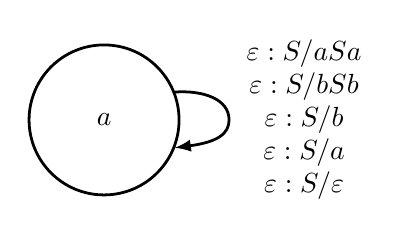
\begin{tikzpicture}[>=latex,line join=bevel,]
  \pgfsetlinewidth{1bp}
%%
\pgfsetcolor{black}
  % Edge: a -> a
  \draw [->] (52.443bp,46.036bp) .. controls (63.028bp,46.728bp) and (72bp,43.383bp)  .. (72bp,36bp) .. controls (72bp,31.155bp) and (68.136bp,28.049bp)  .. (52.443bp,25.964bp);
  \definecolor{strokecol}{rgb}{0.0,0.0,0.0};
  \pgfsetstrokecolor{strokecol}
  \draw (99bp,36bp) node {$\begin{matrix} \varepsilon: S/aSa \\ \varepsilon: S/bSb \\ \varepsilon: S/b \\ \varepsilon: S/a \\ \varepsilon: S/\varepsilon \\ \end{matrix}$};
  % Node: a
\begin{scope}
  \definecolor{strokecol}{rgb}{0.0,0.0,0.0};
  \pgfsetstrokecolor{strokecol}
  \draw (27bp,36bp) ellipse (27bp and 27bp);
  \draw (27bp,36bp) node {$a$};
\end{scope}
%
\end{tikzpicture}



Given $G = \left<V,\Sigma,S,P\right>$ consider the PDA


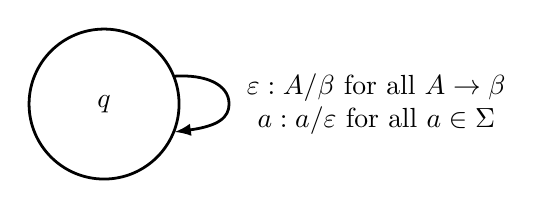
\begin{tikzpicture}[>=latex,line join=bevel,]
  \pgfsetlinewidth{1bp}
%%
\pgfsetcolor{black}
  % Edge: q -> q
  \draw [->] (52.443bp,37.036bp) .. controls (63.028bp,37.728bp) and (72bp,34.383bp)  .. (72bp,27bp) .. controls (72bp,22.155bp) and (68.136bp,19.049bp)  .. (52.443bp,16.964bp);
  \definecolor{strokecol}{rgb}{0.0,0.0,0.0};
  \pgfsetstrokecolor{strokecol}
  \draw (125bp,27bp) node {$ \begin{matrix} \varepsilon: A/\beta \text{ for all } A \to \beta \\ a: a/\varepsilon \text{ for all } a \in \Sigma \\ \end{matrix}$};
  % Node: q
\begin{scope}
  \definecolor{strokecol}{rgb}{0.0,0.0,0.0};
  \pgfsetstrokecolor{strokecol}
  \draw (27bp,27bp) ellipse (27bp and 27bp);
  \draw (27bp,27bp) node {$q$};
\end{scope}
%
\end{tikzpicture}



\begin{itemize}
	\item For all rules $A \to \beta$ in the grammar, $\delta(q,\varepsilon,A)$
		include $(q,\beta)$ There are no other members of
		$\delta(q,\varepsilon,)$
	\item For all terminals $a \in T$, $\delta(q,a,a) = \{ (q,\varepsilon)\}$
	\item All other values of $\delta(q,x,g)$ are empty.
\end{itemize}

\end{proof}

\textbf{Theorem}: Given a PDA that accepts by empty state, there exists a CFG
that accepts the same language as the PDA.

\begin{proof}

	$\forall p,q \in Q$ and $X \in \Gamma$, create a non-terminal
	$\left[pXq\right]$.

	$\left[pXq\right]$: corresponds to the following event:
	\begin{itemize}
		\item we are in state $p$ when $X$ is first pushed on to the stack.
		\item We'll be in state $Q$ when it's finally popped off the stack.
	\end{itemize}

	Suppose that one of the productions in $\delta(q,a,X)$ is $(r,Y_1Y_2\cdots
	Y_k)$. Then add a production $[pXq] \to
	a[ry_1r_1][r_1Y_2r_3]\cdots[r_{k-1}Y_kr_k]$ to the grammar, for all choices
	of $r_1,\cdots,r_k$ from our state set $Q$.  \end{proof}

\end{document}
% vim: tw=80
